\begin{enumerate}[label=\thesection.\arabic*.,ref=\thesection.\theenumi]
\numberwithin{equation}{enumi}

\item The open loop transfer function of a system is 
\begin{align}
G(s) = \frac{2}{(s+1)(s+2)}
\label{eq:ee18btech11017_system}
\end{align}
Find its magnitude and phase response.
\\
\solution Substituting $s = \j\omega$ in \eqref{eq:ee18btech11017_system},

\begin{align}
G\brak{\j\omega}&=\frac{1}{\brak{j\omega+1}\brak{j\omega+2}} 
\\
\implies 
\abs{G\brak{\j\omega}}&=\frac{2}{\brak{\sqrt{\omega^2+1}}\brak{\sqrt{\omega^2+4}}}
\label{eq:ee18btech11017_gain}
\\
\angle G\brak{\j\omega}&=- tan^{-1}(\omega) - tan^{-1}\brak{\frac{\omega}{2}} 
\label{eq:ee18btech11017_phase}
\end{align}

\item Find $\omega$ for which the gain of \eqref{eq:ee18btech11017_system} first becomes 1.
\\
\solution From \eqref{eq:ee18btech11017_gain}

\begin{align}
\abs{G\brak{\j\omega}}&==1
\\
\implies \frac{2}{\brak{\sqrt{\omega^2+1}}\brak{\sqrt{\omega^2+4}}}&=1
\\
\implies \omega_{gc}&=0
\end{align}
which is the desired frequency.

\item Find $\angle G(\j\omega_{gc}) + 180\degree$.  This is known as the {\em phase margin}(PM)
\solution From \eqref{eq:ee18btech11017_phase},
%
\begin{align}
\angle G\brak{\j\omega} = 0\degree
\implies PM=180\degree
\end{align}
%
\item Verify your result by plotting the gain and phase plots of $G(\j\omega)$.
\begin{lstlisting}
codes/ee18btech11017.py
\end{lstlisting}
\item
The Phase plot is as shown,
\begin{figure}[!h]
  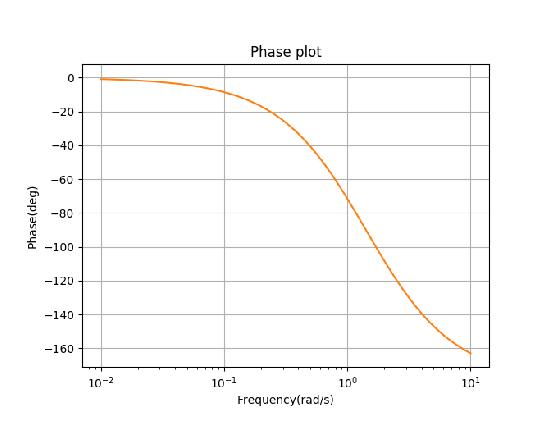
\includegraphics[width=\columnwidth]{./figs/ee18btech11017/ee18btech11017.eps}
  \caption{}
  \label{fig:ee18btech11017}
\end{figure}
\item
\textbf{Application:} 
Phase margin is measure of stability in closed-loop, dynamic-control systems.(i.e, For stability of a system both gain margin and phase margin should be positive.)
\item
\textbf{Example:}Phase Margin is a measure of stability. \\
Consider a unity negative feedback system with open loop gain ,
\\
\begin{align}
G(s)=\frac{10000}{s(s+10)^{2}}
\label{eq:3} 
\end{align}
We can find mgnitude and phase as \\
\begin{align}
|G(j\omega)|=\frac{10^{4}}{\omega \sqrt{(\omega^{2}+10^{2})^{2}}} \\
\angle G(j\omega)=-90^{\circ}-2tan^{-1}\frac{\omega}{10} \label{eq:5} 
\end{align}
At the gain cross over frequency $\omega_{gc}$,$|G(j\omega)|=1$
\\
\begin{align}
\frac{10^{4}}{\omega_{gc} \sqrt{(\omega_{gc}^{2}+10^{2})^{2}}}=1 \\
\end{align}
Simplifying we get,
\begin{align}
\omega_{gc}^{3}+10^{2}\omega_{gc}-10^{4}=0 \\
=> \omega_{gc}=20,-10+20j,-10-20j
\end{align}
As frequency is a real quantity
\\Hence, $\omega_{gc} \neq$ Imaginary
\begin{align}
\therefore  \omega_{gc} =20   \label{eq:6} 
\end{align}
From (\ref{eq:5}) and (\ref{eq:6}) we get,
\begin{align}
P.M=180^{\circ}-90^{\circ}-2tan^{-1}(\frac{\omega_{gc}}{10}) \\
=> P.M=-36.9^{\circ}
\end{align}
We can verify the above result using phase plot.The following code plots Fig(\ref{fig:ee18btech11017_1})
\begin{lstlisting}
codes/ee18btech11017.py
\end{lstlisting}
The Phase plot is as shown,
\begin{figure}[!h]
  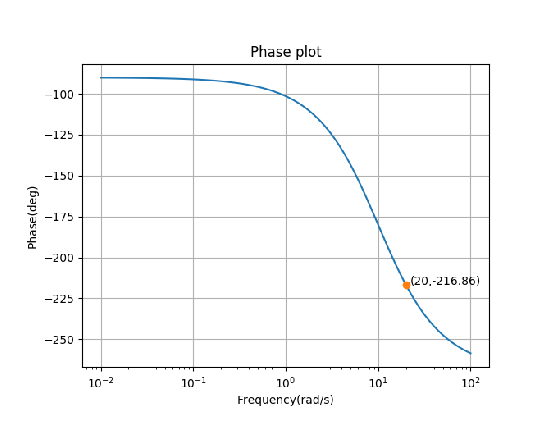
\includegraphics[width=\columnwidth]{./figs/ee18btech11017/ee18btech11017_1.eps}
  \caption{}
  \label{fig:ee18btech11017_1}
\end{figure}
We can observe that at $\omega_{gc}=20$ , $\phi=-216.86^{\circ}$
\\
\begin{align}
\therefore P.M=180^{\circ}+-216.86^{\circ}=-36.9^{\circ} \\
\end{align}
As Phase Margin is negative . Therefore the closed loop system is unstable .
We can verify closed loop stability using Routh-Hurwitz criterion.


\item
Verifying the above example using Routh-Hurwitz criterion.\\
Let $T(s)$ be Closed loop transfer function ,
\begin{align}
T(s)=\frac{N(s)}{D(s)}=\frac{G(s)}{1+G(s)}
\end{align}
The characteristic equation is 
\begin{align}
D(s)=0  \\
1+G(s)=0 
\end{align}

\begin{align}
=> s^{3}+20s^{2}+100s+10000=0   \label{eq:7} 
\end{align}
\\
Constructing routh array for (\ref{eq:7})..,
\begin{align}
\mydet{s^3\\s^2\\s}
\mydet{1 & 100 & 0 \\ 20 & 10000 & 0 \\ -400 & 0 & 0}
\end{align}\\

\begin{align}
\mydet{s^3\\s^2\\s\\s^0}
\mydet{1 & 100 & 0 \\ 20 & 10000 & 0 \\ -400 & 0 & 0 \\ 10000 & 0 & 0}
\end{align}\\

There are two sign changes in the first column of the routh array. So, two poles lie on right half of s-plane. \\
Therefore,the system is unstable.\\
The following code generates routh array.
\begin{lstlisting}
codes/RouthHurwitz.py
\end{lstlisting}























\end{enumerate}
